% *********************************************************************
% © 2010–2022 Jeremy Sylvestre
%
% Permission is granted to copy, distribute and/or modify this document
% under the terms of the GNU Free Documentation License, Version 1.3 or
% any later version published by the Free Software Foundation; with no
% Invariant Sections, no Front-Cover Texts, and no Back-Cover Texts. A
% copy of the license is included in the appendix entitled “GNU Free
% Documentation License” that appears in the output document of this
% PreTeXt source code. All trademarks™ are the registered® marks of
% their respective owners.
%
% *********************************************************************

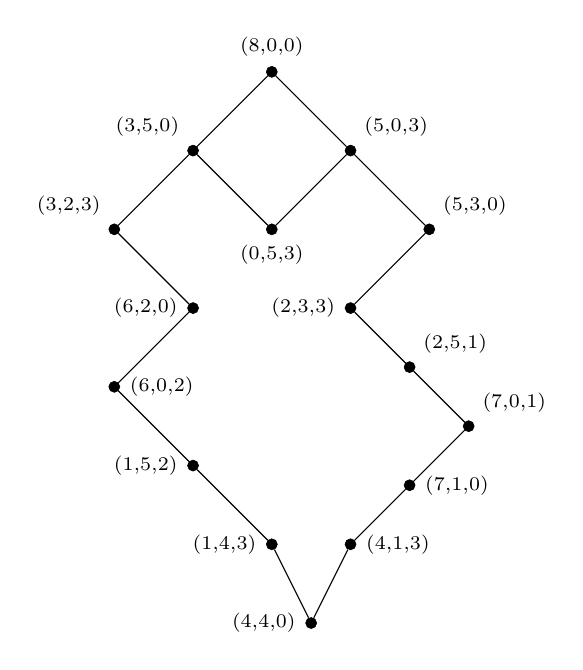
\begin{tikzpicture}[
	vertex/.style={ circle, draw, very thin, fill, inner sep=0pt, minimum size=4pt },
	vertexg/.style={ black!40!white, circle, draw, very thin, fill, inner sep=0pt, minimum size=4pt },
	vertexo/.style={ circle, draw, very thin, inner sep=0pt, minimum size=4pt }
]

\node at (0,8) (p800) [vertex,label=above:{$\scriptstyle (8,0,0)$}] {};

\node at (-1,7) (p350) [vertex,label=above left:{$\scriptstyle (3,5,0)$}] {};
\draw (p350) to (p800);

\node at (1,7) (p503) [vertex,label=above right:{$\scriptstyle (5,0,3)$}] {};
\draw (p503) to (p800);

\node at (0,6) (p053) [vertex,label=below:{$\scriptstyle (0,5,3)$}] {};
\foreach \p in {p350,p503} \draw (p053) to (\p);

\node at (-2,6) (p323) [vertex,label=above left:{$\scriptstyle (3,2,3)$}] {};
\draw (p350) to (p323);

\node at (2,6) (p530) [vertex,label=above right:{$\scriptstyle (5,3,0)$}] {};
\draw (p530) to (p503);

\node at (-1,5) (p620) [vertex,label=left:{$\scriptstyle (6,2,0)$}] {};
\draw (p620) to (p323);

\node at (1,5) (p233) [vertex,label=left:{$\scriptstyle (2,3,3)$}] {};
\draw (p233) to (p530);

\node at (-2,4) (p602) [vertex,label=right:{$\scriptstyle (6,0,2)$}] {};
\draw (p602) to (p620);

\node at (1.75,4.25) (p251) [vertex,label=above right:{$\scriptstyle (2,5,1)$}] {};
\draw (p251) to (p233);

\node at (-1,3) (p152) [vertex,label=left:{$\scriptstyle (1,5,2)$}] {};
\draw (p152) to (p602);

\node at (2.5,3.5) (p701) [vertex,label=above right:{$\scriptstyle (7,0,1)$}] {};
\draw (p701) to (p251);

\node at (0,2) (p143) [vertex,label=left:{$\scriptstyle (1,4,3)$}] {};
\draw (p143) to (p152);

\node at (1.75,2.75) (p710) [vertex,label=right:{$\scriptstyle (7,1,0)$}] {};
\draw (p710) to (p701);

\node at (0.5,1) (p440) [vertex,label=left:{$\scriptstyle (4,4,0)$}] {};
\draw (p440) to (p143);

\node at (1,2) (p413) [vertex,label=right:{$\scriptstyle (4,1,3)$}] {};
\foreach \p in {p710,p440} \draw (p413) to (\p);

\end{tikzpicture}
